\section{Answers}

\begin{enumerate}
\item Which of the following statements, regarding the usefulness of particle filters, are true?

\begin{enumerate}
\item Particle filters are useful as they can handle almost any models
\item Particle filters are useful as within reasonable computational complexity, the particle filter always gives us the best performance. 
\item Particle filters are useful as they give us a compact description of the posterior density. 
\item Particle filters are useful as they give a non-parametric description of the posterior.
\end{enumerate}

\textbf{Answer:}

The main advantage with particle filters is that they offer a non-parametric description of our posterior. As a consequence of this, it can be used to handle almost any model as long as we can evaluate them point-wise. However, it is hard to argue that we get a compact description of our posterior as we typically use a couple of thousand parameters or even more. Further, it is not a solution that should be used to solve all problems, for example, if we have linear and Gaussian models we should use the ordinary Kalman filter we know that this gives us the optimal solution. So correct options are A and D.
\item Assuming that we describe our posterior using the following approximation
\begin{equation}
p(\mathbf{x}_k | \mathbf{y}_{1:k}) \approx \sum_{i=1}^N w_{k}^{(i)} \delta (\mathbf{x}_k -\mathbf{x}_{k}^{(i)})
\end{equation}

what is the MMSE estimate of $\mathbf{x}_k$?
\begin{enumerate}
\item $\hat{\mathbf{x}}_k = \sum_{i}^{N} w_{k}^{(i)} \mathbf{x}_{k}^{(i)}$
\item $\hat{\mathbf{x}}_k = \mathbf{x}_{k}^{(j)} ~~ \text{where} ~~ j = argmax_i w_{k}^{(i)}$
\item $\hat{\mathbf{x}}_k = \frac{1}{N}\sum_{i}^{N}  \mathbf{x}_{k}^{(i)}$
\item It is not possible to calculate a MMSE estimate from this approximation. 
\end{enumerate}

\textbf{Answer:}

We can view the particle filter representation as approximating the posterior PDF with a posterior PMF where the weight, $w_{k}^{(i)}$, 
gives us the discrete probability that the state is $\mathbf{x}_{k}^{(i)}$, Using the definition of expected value on this PMF gives us the solution above. 
So the correct answer is option A.

\item Consider Figure \ref{P0_7_3_4_ex1}.

\begin{figure}[!htb]
\begin{center}
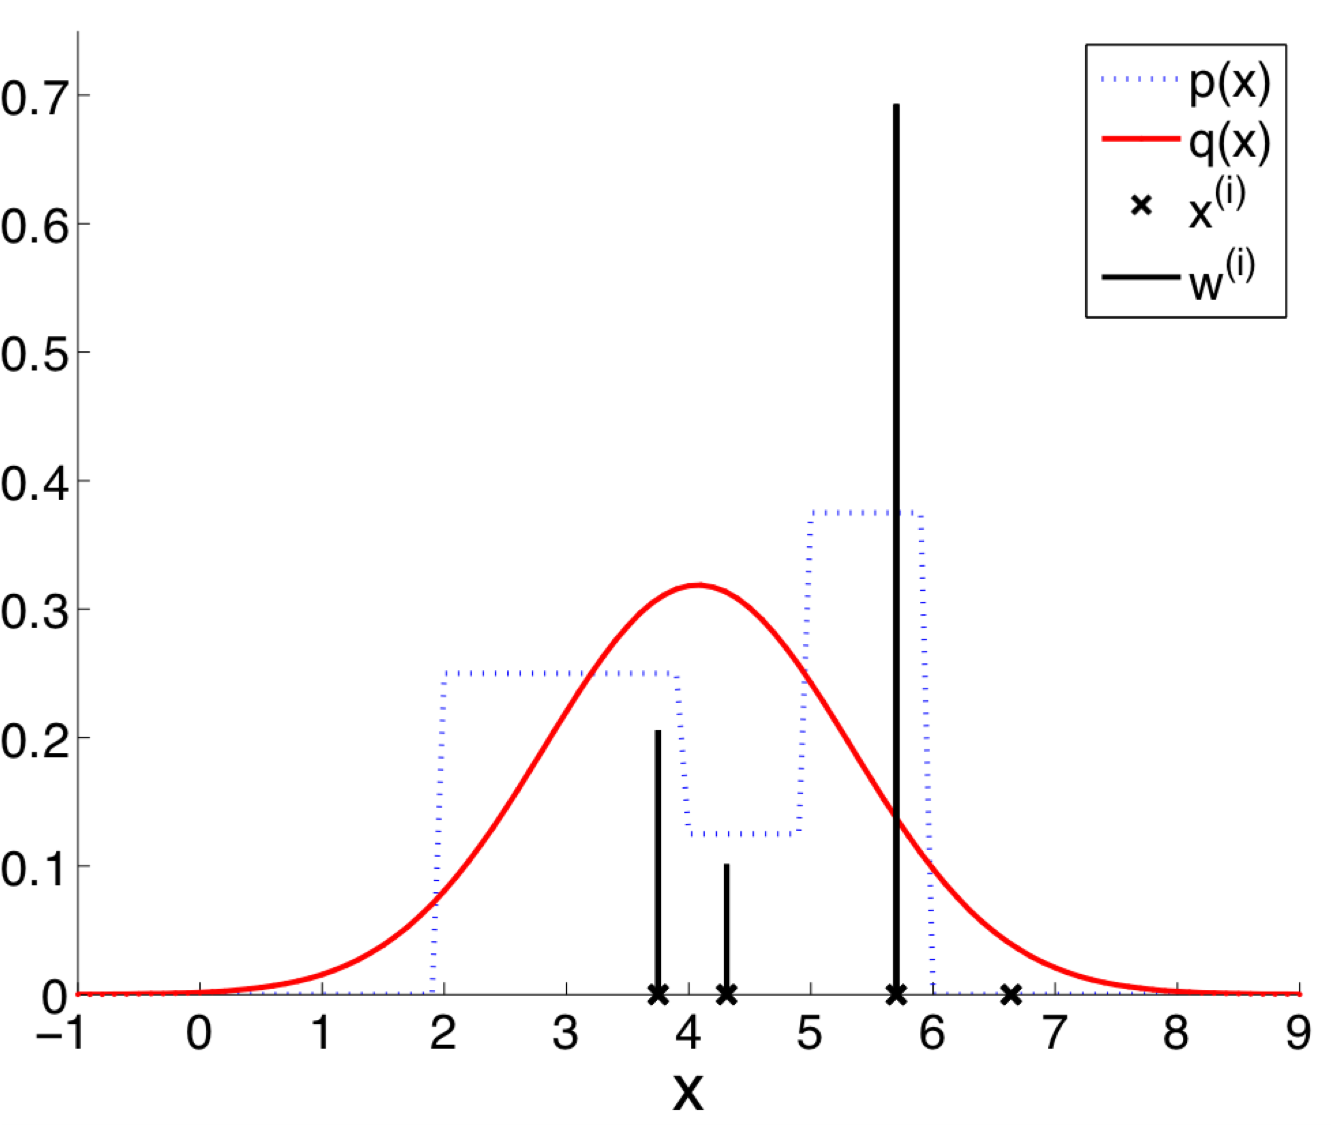
\includegraphics[scale=0.280]{img/particle_filters/P0_7_3_4_ex1.png}
\end{center}
\caption{Question figure.}
\label{P0_7_3_4_ex1}
\end{figure}
Perform resampling on the density and illustrate the result. Assume that the numbers 0.65, 0.03, 0.84 and 0.93 are drawn uniformly from $[0,1]$.
Which one of the following figures illustrates the resampled particles?

\begin{enumerate}
\item \begin{figure}[!htb]
\begin{center}
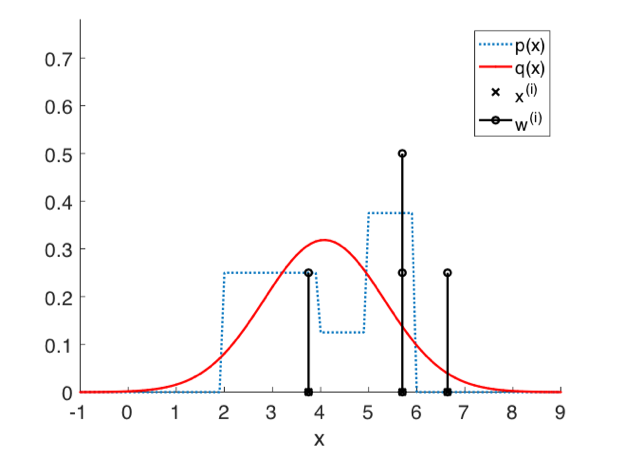
\includegraphics[scale=0.320]{img/particle_filters/P1_7_3_4_ex1.png}
\end{center}
\label{P1_7_3_4_ex1}
\end{figure}
\item \begin{figure}[!htb]
\begin{center}
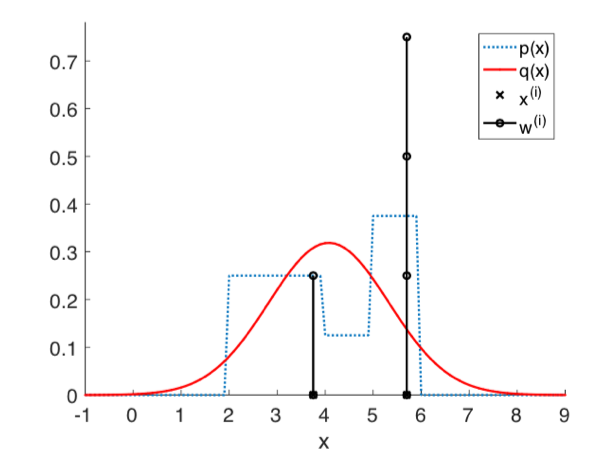
\includegraphics[scale=0.320]{img/particle_filters/P2_7_3_4_ex1.png}
\end{center}
\label{P2_7_3_4_ex1}
\end{figure}
\item \begin{figure}[!htb]
\begin{center}
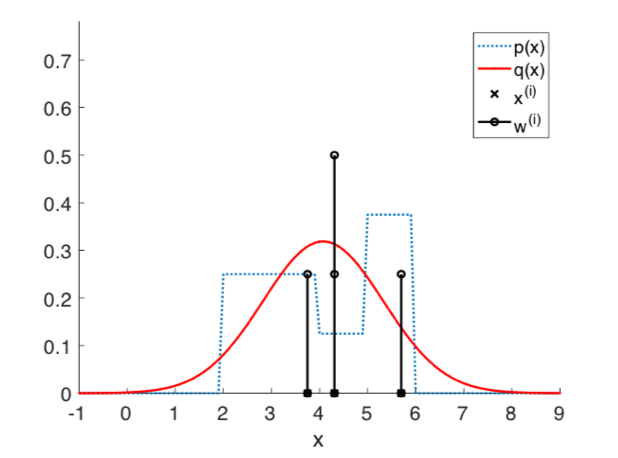
\includegraphics[scale=0.320]{img/particle_filters/P3_7_3_4_ex1.png}
\end{center}
\label{P3_7_3_4_ex1}
\end{figure}
\end{enumerate}

\textbf{Answer:}

If particles are ordered in ascending order, $x^{(1)} < \ldots < x^{(4)}$ resampling gives the following $x^{(1)} = 3.8$ and $x^{(2)} = x^{(3)} = x^{(4)} = 5.7$. Thus, option B is the correct answer.
\end{enumerate}

